\appendix

\chapter{SCREENSHOTS}
\label{app:screenshots}
This appendix presents interface screenshots and physical hardware photographs illustrating the implementation and operation of the Edge-AI Autonomous RC Car platform.

\begin{figure}[H]
\centering
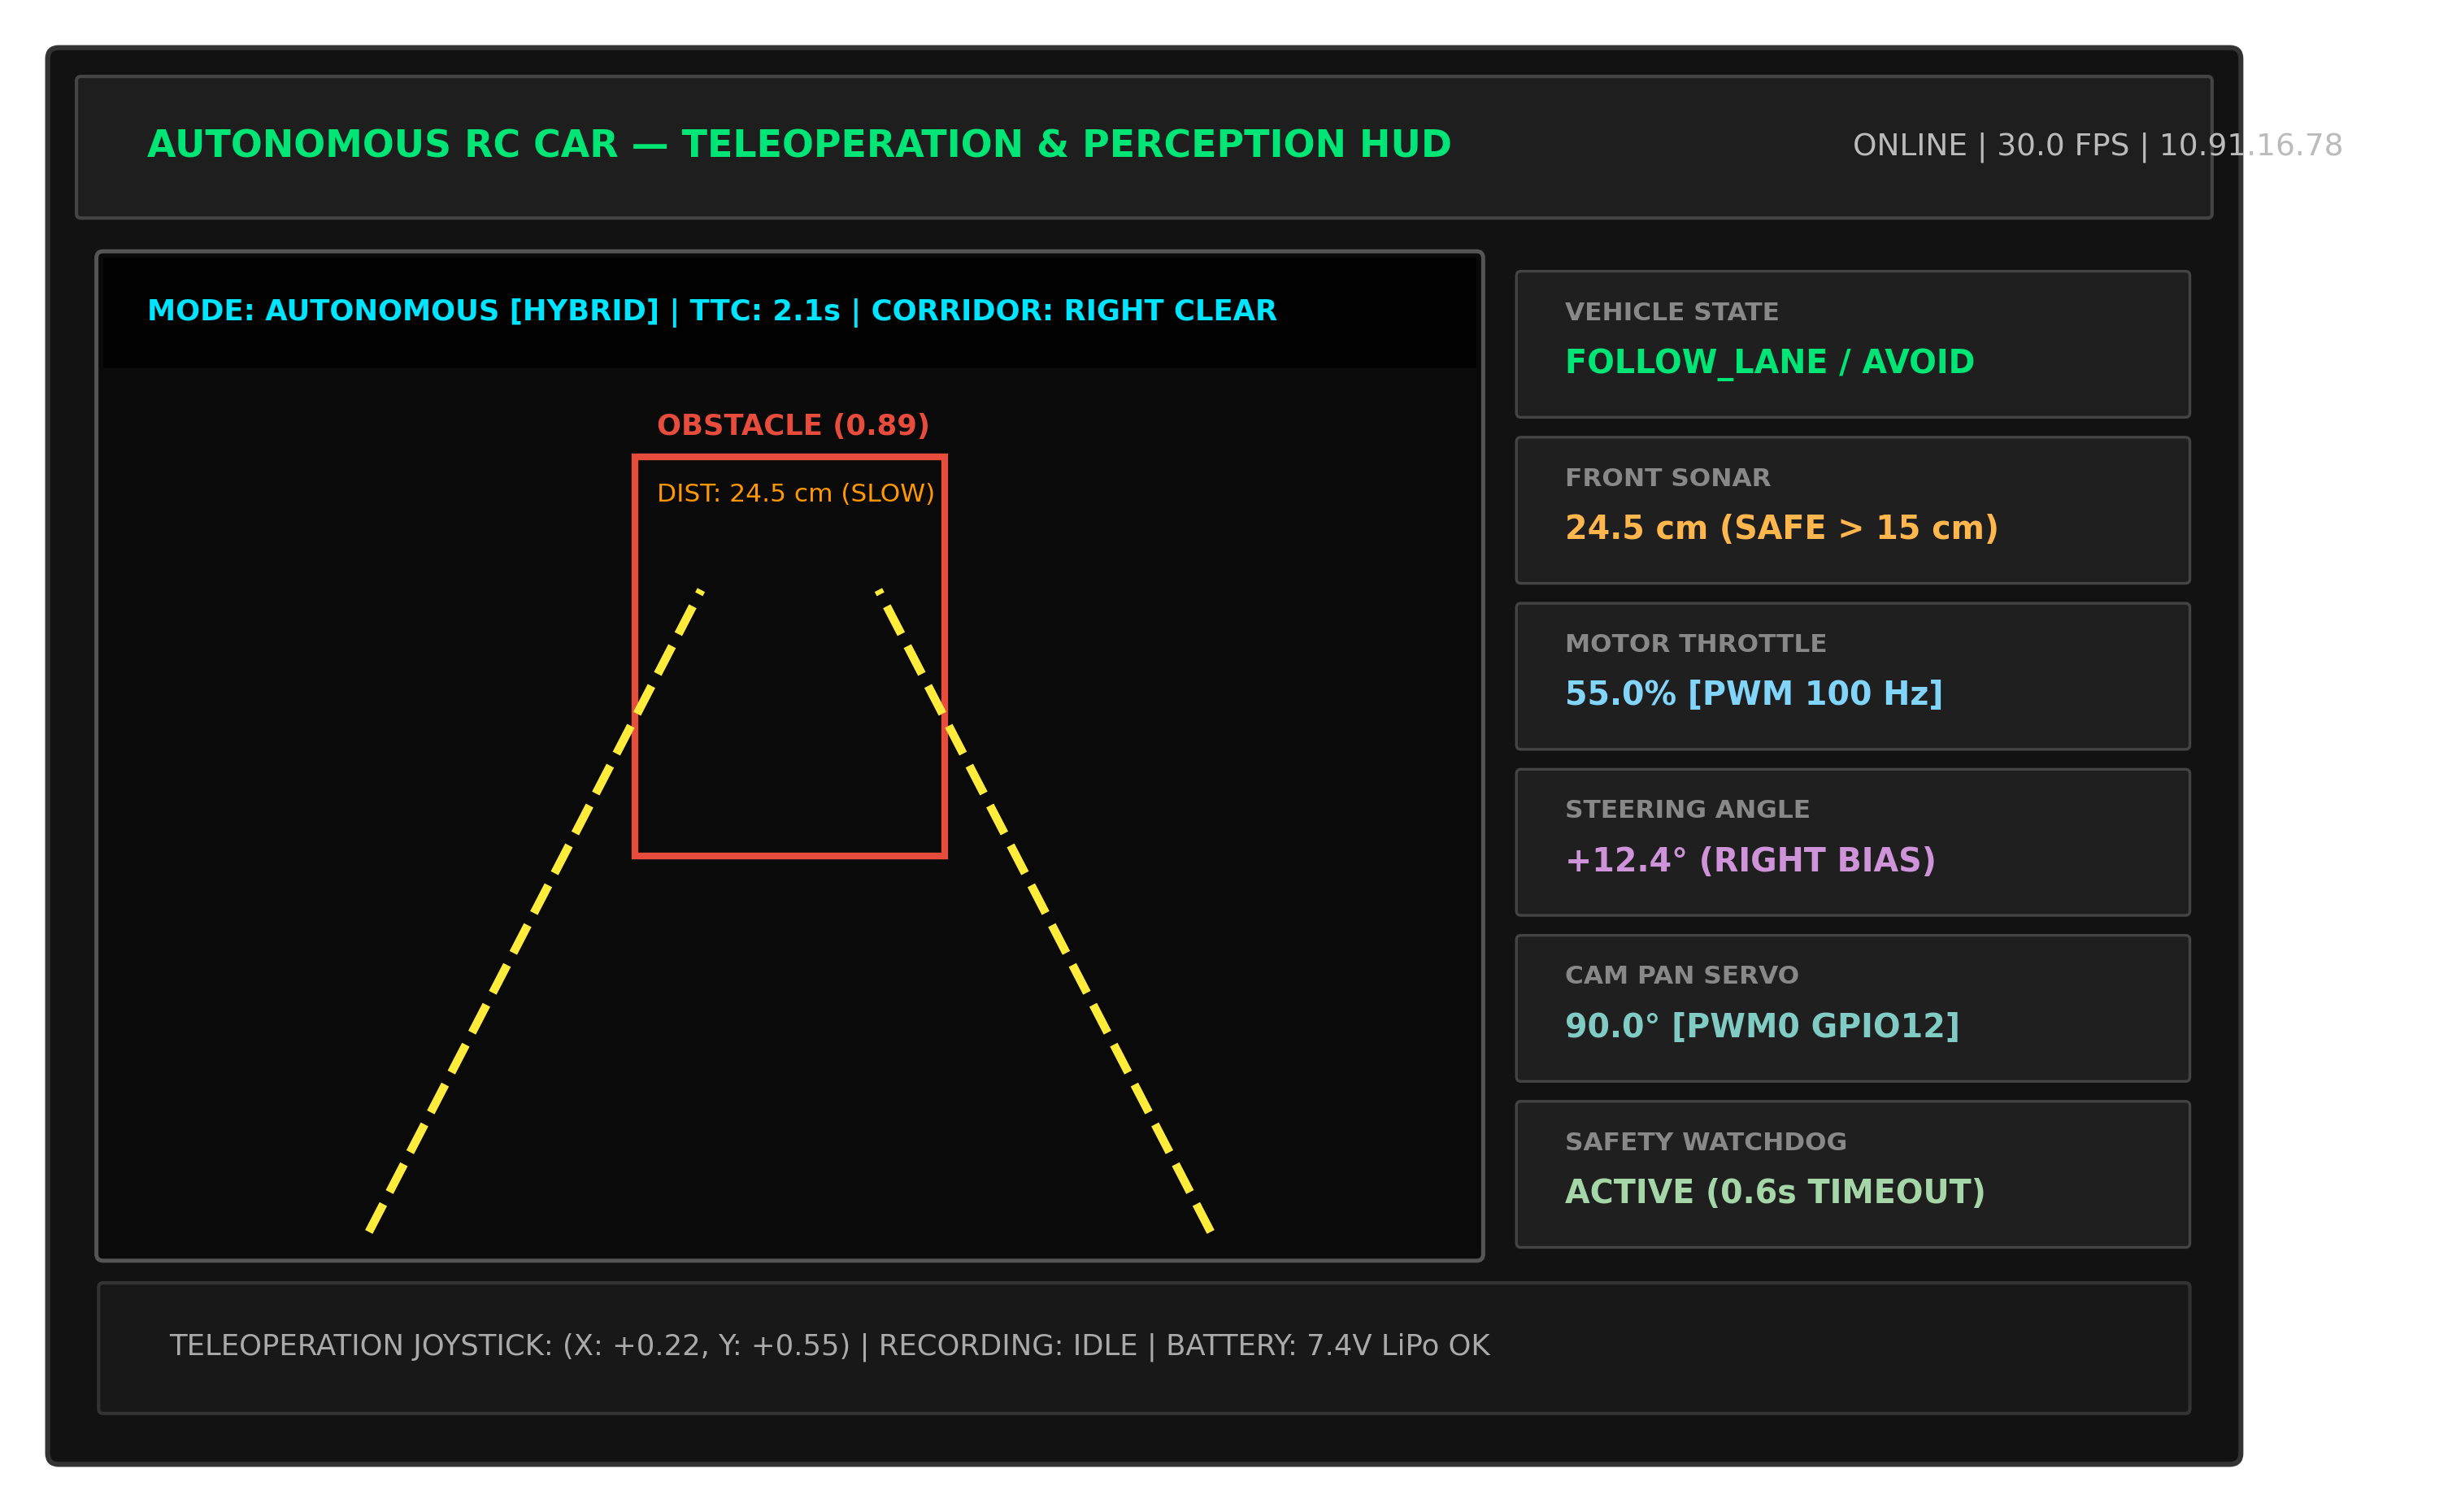
\includegraphics[width=0.92\textwidth]{assets/dashboard_hud.png}
\caption{Screenshot of the Responsive Teleoperation Web Dashboard and Camera HUD Overlay}
\label{fig:app_dashboard}
\end{figure}

Figure~\ref{fig:app_dashboard} shows the Apple-monochrome responsive telemetry dashboard served by Flask on port 5000. The interface renders the real-time MJPEG camera stream annotated with lane trajectory centroids, LiteRT YOLOv8 bounding boxes, looming Time-to-Collision (TTC) metrics, and clear-path corridor meters alongside active ultrasonic distance readouts and directional drive commands.

\begin{figure}[H]
\centering
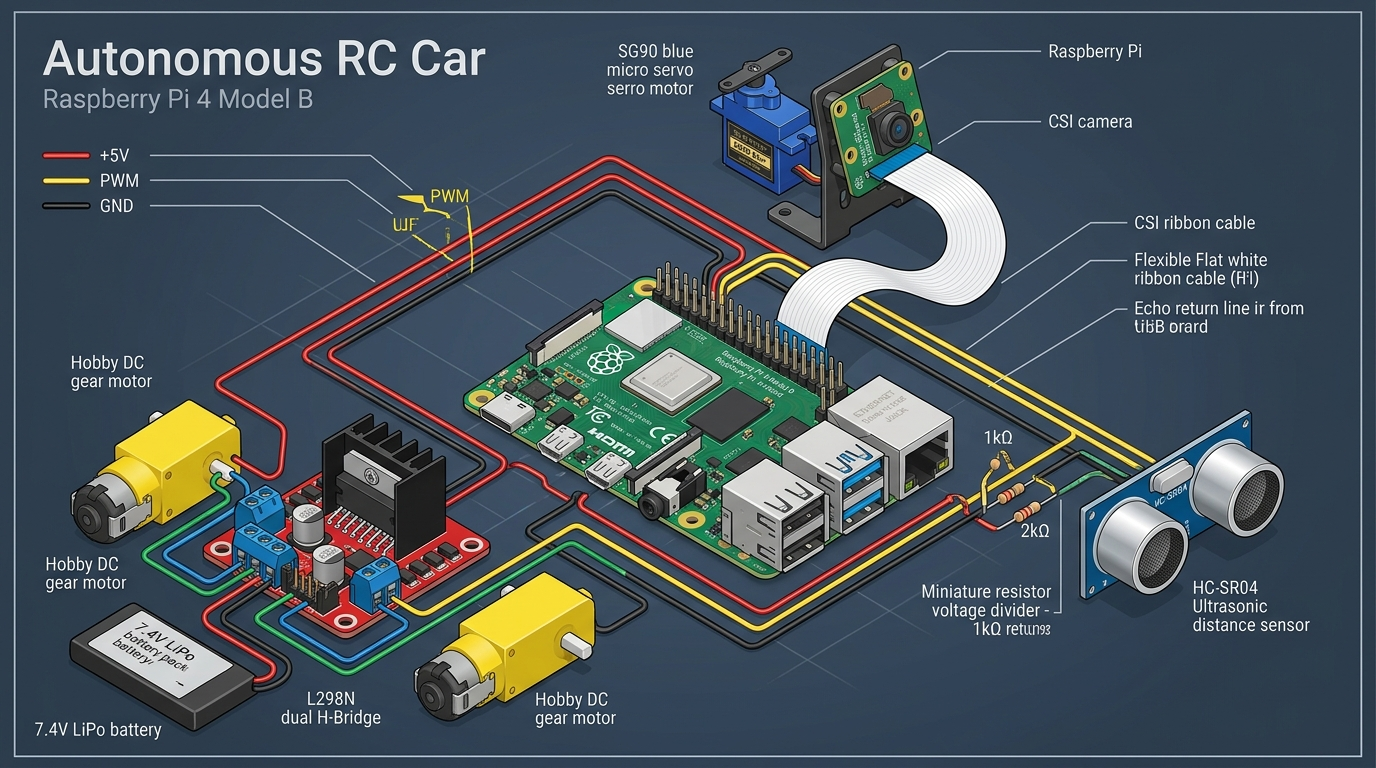
\includegraphics[width=0.88\textwidth]{assets/chassis_wiring.jpg}
\caption{Physical Hardware Assembly, Chassis Architecture, and Sensor Wiring Setup}
\label{fig:app_hardware}
\end{figure}

Figure~\ref{fig:app_hardware} illustrates the physical vehicle chassis, displaying the Raspberry Pi single-board computer, L298N dual H-bridge motor driver, front-mounted HC-SR04 ultrasonic range sensor, SG90 camera survey pan servo, and CSI camera module.

\chapter{SAMPLE CODE}
\label{app:code}
The following Python source code excerpts demonstrate the core implementation of the vehicle's perception loop, differential motor kinematics, and deterministic safety arbiter.

\section{Autonomous Driver Loop and Hazard Arbitration}
The following script excerpt from \texttt{navigation/autonomous\_driver.py} coordinates frame perception, LiteRT YOLOv8 object detection, corridor clearance evaluation, and PID steering.

\begin{lstlisting}[language=Python]
class AutonomousDriver:
    """Master perception and navigation loop running at 30 Hz."""
    def __init__(self, config, motors, servo, camera, safety_arbiter):
        self.config = config
        self.motors = motors
        self.servo = servo
        self.camera = camera
        self.safety_arbiter = safety_arbiter
        self.detector = TFLiteDetector(config.model_path)
        self.corridor_scanner = CorridorScanner()
        self.pid = PIDController(kp=0.45, ki=0.001, kd=0.12)

    def step(self):
        # 1. Grab latest camera frame
        frame = self.camera.get_bgr_frame()
        if frame is None:
            return

        # 2. Extract lane guidance error via contour moments
        lane_result = detect_lane_centroid(frame)
        steering_corr = self.pid.compute(lane_result.error)

        # 3. Perform edge AI detection and corridor sector density scan
        detections = self.detector.infer(frame)
        corridor = self.corridor_scanner.evaluate_sectors(frame)

        # 4. Formulate candidate motion command
        throttle = self.config.cruise_speed
        if corridor.hazard_detected:
            throttle = self.config.avoid_speed
            steering_corr = corridor.suggested_evasion_bias

        # 5. Pass motion authority to Safety Arbiter
        safe_action = self.safety_arbiter.evaluate_action(
            throttle=throttle, steering=steering_corr
        )
        self.motors.drive(safe_action.throttle, safe_action.steering)
\end{lstlisting}

\section{Proportional Differential Tank-Mix Motor Controller}
The following script from \texttt{hardware/motors.py} drives the L298N H-bridge using software PWM at 100~Hz with dual IN2 pin mirroring and a 0.6-second watchdog auto-stop timer.

\begin{lstlisting}[language=Python]
import RPi.GPIO as GPIO
import time

class MotorController:
    """360-degree proportional differential drive with watchdog."""
    def __init__(self, in1=17, in2=27, in3=22, in4=23, in2_alt=18):
        self.in1, self.in2, self.in3, self.in4 = in1, in2, in3, in4
        self.in2_alt = in2_alt
        self.last_command_time = time.time()
        self.watchdog_timeout = 0.6
        self._setup_gpio_pwm()

    def drive(self, throttle: float, steering: float):
        """Computes differential tank-mix wheel velocities."""
        self.last_command_time = time.time()
        v_left = max(-1.0, min(1.0, throttle + steering))
        v_right = max(-1.0, min(1.0, throttle - steering))
        self._apply_pwm(v_left, v_right)

    def check_watchdog(self):
        """Halts motors immediately if control stream drops."""
        if time.time() - self.last_command_time > self.watchdog_timeout:
            self.stop()
\end{lstlisting}

\section{Deterministic Safety Arbiter and Sonar Guard}
The following module from \texttt{control/safety\_supervisor.py} enforces emergency braking whenever front sonar detects an obstacle under 15~cm.

\begin{lstlisting}[language=Python]
class SafetySupervisor:
    """Hard real-time safety gate preventing physical collision."""
    def __init__(self, emergency_distance_cm=15.0):
        self.emergency_distance_cm = emergency_distance_cm

    def validate_motion(self, target_throttle: float, steering: float,
                        front_sonar_reading):
        # Reject stale sensor measurements (>250 ms old)
        if front_sonar_reading is None or front_sonar_reading.is_stale():
            return Action(throttle=0.0, steering=0.0, reason="STALE_SONAR")

        # Emergency override if obstacle within braking threshold
        if front_sonar_reading.distance_cm < self.emergency_distance_cm:
            return Action(throttle=0.0, steering=0.0, reason="EMERGENCY_STOP")

        return Action(throttle=target_throttle, steering=steering, reason="SAFE")

\section{Behavioral Cloning CNN Architecture and Real-Time Pilot Decoder}
The following module from \texttt{behavioral\_cloning.py} demonstrates the on-device ONNX runtime execution, image preprocessing, and the 9-bucket directional steering decoding engine.

\begin{lstlisting}[language=Python]
class PilotModel:
    """Lazy ONNX/LiteRT adapter with 9-bucket directional steering decoder."""
    def __init__(self, model_path: str = "models/SidewalkPilot-v3.1b.onnx"):
        self.model_path = model_path
        self._session = None

    def load(self) -> bool:
        import onnxruntime as ort
        opts = ort.SessionOptions()
        opts.intra_op_num_threads = 2
        opts.graph_optimization_level = ort.GraphOptimizationLevel.ORT_ENABLE_ALL
        self._session = ort.InferenceSession(self.model_path, opts, providers=["CPUExecutionProvider"])
        return True

    def predict(self, frame: np.ndarray) -> Tuple[float, float]:
        """Preprocesses 640x480 frame and runs ONNX inference."""
        # 1. Resize to 200x66 DAVE-2 input and normalize (-1.0 to +1.0)
        img = cv2.resize(frame, (200, 66), interpolation=cv2.INTER_AREA)
        tensor = ((img.astype(np.float32) / 255.0 - 0.5) / 0.5).transpose(2, 0, 1)
        batch = np.expand_dims(tensor, axis=0)

        # 2. Run inference session on ARM Cortex-A72
        raw = self._session.run(None, {self._session.get_inputs()[0].name: batch})[0].reshape(-1)

        # 3. Decode 19-dimensional SidewalkPilot output vector
        # First 9 elements: Softmax classification logits for 20-deg sectors
        bucket = int(np.argmax(raw[:9]))
        fraction = 1.0 / (1.0 + math.exp(-float(raw[9 + bucket])))
        
        # Linear interpolation within active 20-deg bucket
        angle_deg = bucket * 20.0 + fraction * 20.0
        steering = max(-1.0, min(1.0, (angle_deg - 90.0) / 90.0))
        throttle = max(0.0, min(1.0, 1.0 / (1.0 + math.exp(-float(raw[18])))))
        return steering, throttle
\end{lstlisting}
